\chapter{Introduction}
%\label{chap:GettingStarted}

\section{Introduction}
%\label{sec:ChoosingAdvisor}
Software cost models and effort approximations support project supervisors to distribute resources, control budgets and agenda and develop modern practices, leading to projects completed on time and within financial plan. If cost and effort are determined suspicious in software projects, suitable occasions can be missed; whereas expectant predictions can be affected to some resource losing. In the context of web development, these issues are also vital and very challenging given that web projects have short schedules and very fluidic opportunity. Since software projects are continually changed in nature, earlier projects may not necessarily cover all aspects of a new project when used as a basis for cost estimation. Preliminary software estimation models are constructed on regression analysis or mathematical sources.
\section{System Review}

In this arena, some applications are run sequentially. Some of them are – OpenConf, OCS,EasyChair,CMT etc.Some
Modules of this System: Acceptance,Bidding,Discussion
Form Fields,CAPTCHA,File Type, Proceedings.\newline
\textbf{OpenConf:}Install system, check configuration and enable modules, open submission,
 upload and reviewer signup, assign reviewers and advocates, decision and notification.\cite{ref2}\newline
In OpenConf,there has no support to create multi-conference system,payment method
,Website creation,A/R paper download option,speaker scheduling.\newline

\textbf{OCS(Open Conference System):} Open Conference Systems (OCS) is a free Web publishing tool that will create a complete Web presence for your scholarly conference.OCS will allow you to:create a conference web site,compose and send a call for papers,electronically accept paper and abstract submissions,allow paper submitters to edit their work,post conference proceedings and papers in a searchable format,post,if you wish,the original data sets,register participants,integrate post-conference online discussions.\cite{ref3}\newline
In OCS, there has no support to create IEEE eCopyright,Website creation,A/R paper download option,sponsor tracking and speaker scheduling.\newline
\textbf{CMT: Microsoft’s Academic Conference Management Service-} The Conference Management Toolkit (CMT) is a free conference management service sponsored by Microsoft Research.CMT is capable of handling the complex workflow of an academic conference including:Customizable paper submission, reviewer,and author feedback forms,Author notification,Review submission etc.\cite{ref6}\newline
In CMT, there has no support to create multi-conference system,support multiple paper submission in one account,payment method,Website creation,A/R paper download option.\newline
\textbf{EasyChair:} EasyChair is a conference management system that is flexible, easy to use, and has many features to make it suitable for various conference models\cite{ref4}\newline
In EasyChair, there has no support to create multi-conference system,IEEE eCopyright,payment method,Website creation,A/R paper download option.\newline
Comparison above all systems with ProConf according to free addition.Such as:\newline

\begin{center}
\begin{table}[htbp]
   \begin{tabular}{|c|c|c|c|c|c|}
     \hline
     % after \\: \hline or \cline{col1-col2} \cline{col3-col4} ...
     Topics & ProConf & OpenConf & OCS & EasyChair & CMT \\\hline
     Make Submission & Y & Y & Y & Y & Y \\\hline
     Allow Multiconference & Y & N & Y & Y & N\\\hline
     Payment System & Y &N & Y & N & N  \\\hline
     Create Website  & Y & N & Y & N & N \\\hline
     P/N Author Registration & Y & Y & N & N & N \\\hline
     IEEE eCopyright & Y & N & N & N & Y \\\hline
     A/R paper Download option & Y & N & N & N & N\\\hline
     Program  Schedule Creation & Y &N & N & N & N \\\hline
     Online Registration & Y & Y & Y & y & Y\\\hline
     Speaker scheduling & Y & N & N & N & N\\\hline
     Multi-track support & Y & N & N & Y & N\\\hline
     MPS in one account & Y & N & N & N& N\\\hline
     Track Assign       &Y &N &N &Y &N \\\hline
     PM with RFID & Y & N & N & N & N\\\hline



   \end{tabular}
   \caption[Comparison with Existing System.]{Comparison with Existing System}
	\label{tab:comparison}

  \end{table}
  \end{center}


\section{Proposed  System }
Identify these problems, this proposed system target is to overcome those problems. Primarily, The Proposal entitled as ProConf can do Peer-Review, Abstract and Conference Management.ProConf is a free Web publishing tool that will create a complete Web presence for scholarly conference.
Proconf covers all aspects of online conference management and publishing, from setting up conference website to operational tasks such as submitting, reviewing, editing, publishing, archiving, and indexing of the conference papers.
Proconf also helps to manage the people involved in organizing a conference, reviewers, and authors,notifying readers and registrants, and assisting with the correspondence. Additionally, Payment system module is added and free as open source to anyone. In existing all conference system there has no concept of RFID. Main featured of proposed system is helpful to program management with RFID technologies.\newline
Below, there is an overview of the process ProConf uses.
\begin{center}
\begin{table}[htbp]
   \begin{tabular}{|c|c|c|c|c|c|}
     \hline
     % after \\: \hline or \cline{col1-col2} \cline{col3-col4} ...
     Topics &Chair &TC/C-C/M &Author & Reviewer & P/N \\\hline
     Install and Config &Y & N & N &N &N \\\hline
     Create Website & Y & N & N &N &N \\\hline
     Open and Close Submissions& Y & N & N &N &N \\\hline
     Sign-Up & N & Y & Y &Y &Y \\\hline
     Decision  and Notification & Y & N & N &N &N \\\hline
     CCPM & Y & N & N &N &N \\\hline
     Assign  Reviewers & Y & Y & N & N & N \\\hline
     OCRS & Y & N & N & N & N \\\hline
     Review Submission & N & Y & N & Y & N \\\hline
     PM with RFID  & Y & N & N & N & N \\\hline
     Give Comment after review  & N & TC-Y & N & N & N \\\hline
   \end{tabular}
   \caption[Proposed System Process.]{Proposed System Process}
	\label{tab:system process}

  \end{table}
  \end{center}







\section{System overview}
 ProConf is an open source multi-conference system to manage and publish online conferences. ProConf shields all aspects of available conference management and publishing, from setting up conference website to operational tasks such as submitting, reviewing, editing, publishing, archiving, and indexing of the conference papers. ProConf also helps to manage the people involved in organizing a conference, reviewers and authors, notifying readers and registered participants and assisting with the correspondence. Program Schedule, Conference Paper publish, Conference website development, Payment module etc are the main feature of this proposal. It has been designed to shrink the time and energy fanatical to the secretarial and executive tasks related with supervision of a online conference, while refining the record-keeping and efficiency of editorial processes.\newline
Additionally, ProConf is flexible and scalable. A single installation of ProConf can support the operation of multiple conferences, and multiple years for each conference. Each conference has its own unique URL as well as its own look and feel. ProConf can enable a single director to manage all aspects of a conference. At last, it is an open source helpline for anyone who conduct any online conference.


\begin{figure}[h!]
\centering
  % Requires \usepackage{graphicx}
  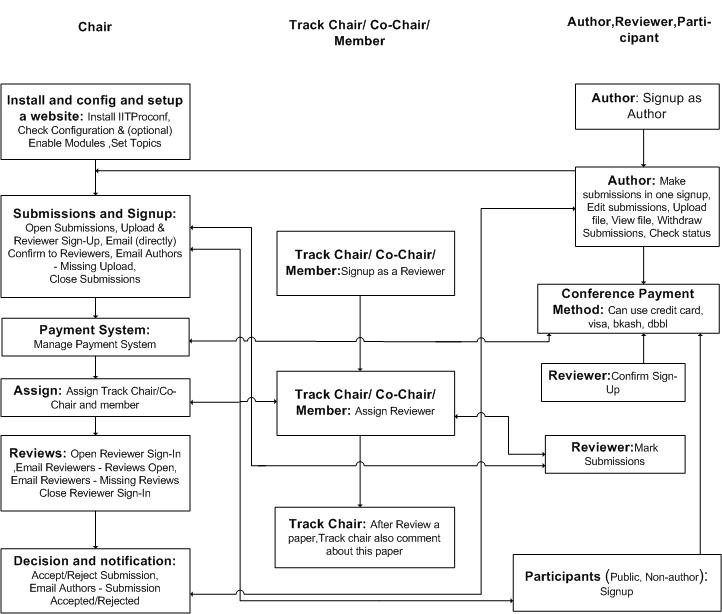
\includegraphics[width=5in]{pic/review}
  \caption{System Overview}\label{system}
\end{figure}


\section{Methodology}

\begin{enumerate}
  \item The research approach try to introduce dataset includes basic requirements of projects with some Functional Measurement types and complexity Factor of the software development effort. So, using dataset for evaluating the proposed model is based on Algorithmic model.
  \item The second attempt will to create an all requirement dataset based on one of requirement, based on model and algorithm.
  \begin{itemize}
    \item Estimate criteria for each requirement in dataset, then asserts it into several equal intervals (lengths).
    \item Cost Factor matrix development
    \item Estimate a corresponding extra linguistic variable for each interval of requirement of Functional Measurement Type.
    \item Estimate Project management software primary functions
  \end{itemize}
\end{enumerate}

\section{Socio-Economic Importance}

\begin{itemize}
  \item Help supervisor to manage resources, control budgets and agenda and develop modern practices.
  \item Help Project Managers to complete on time and within financial plan.
  \item Make better relationship between Software clients and Project Managers \& Developers.
  \item Financial Report generate for Clients satisfaction.
\end{itemize}


\section{Time Frame}

% Please add the following required packages to your document preamble:
% \usepackage{multirow}
% \usepackage[table,xcdraw]{xcolor}
% If you use beamer only pass "xcolor=table" option, i.e. \documentclass[xcolor=table]{beamer}
% \usepackage[normalem]{ulem}
% \useunder{\uline}{\ul}{}
\begin{table}[h!]
\centering
\caption{Time Frame (March 2015 - December 2015)}
\label{time_frame_mar_2015}
\begin{tabular}{|l|l|l|l|l|l|l|l|l|l|l|}
\hline
\multicolumn{1}{|c|}{}                                                                                                             & \multicolumn{10}{c|}{2015}                                                                                                                                                                                                                                                  \\ \cline{2-11}
\multicolumn{1}{|c|}{\multirow{-2}{*}{\textbf{Activity}}}                                                                          & Mar                      & Apr                      & May                      & Jun                      & Jul                      & Aug                      & Sep                      & Oct                      & Nov                      & Dec                      \\ \hline
\multicolumn{11}{|l|}{\cellcolor[HTML]{C0C0C0}\textit{Preparations \& Study}}                                                                                                                                                                                                                                                                                                                                    \\ \hline
\begin{tabular}[c]{@{}l@{}}Activity 1.1 Explore \\ Software Cost And \\ Effort Estimation Models\end{tabular}                      & \cellcolor[HTML]{68CBD0} & \cellcolor[HTML]{68CBD0} &                          &                          &                          &                          &                          &                          &                          &                          \\ \hline
\begin{tabular}[c]{@{}l@{}}Activity 1.2 Development \\ of dataset for \\ Software Cost\end{tabular}                                &                          & \cellcolor[HTML]{68CBD0} & \cellcolor[HTML]{68CBD0} &                          &                          &                          &                          &                          &                          &                          \\ \hline
\begin{tabular}[c]{@{}l@{}}Activity 1.3 Data \\ Collection form \\ Industrial Mentor\end{tabular}                                  &                          &                          & \cellcolor[HTML]{68CBD0} & \cellcolor[HTML]{68CBD0} &                          &                          &                          &                          &                          &                          \\ \hline
\multicolumn{11}{|l|}{\cellcolor[HTML]{C0C0C0}\textit{Development of Approach}}                                                                                                                                                                                                                                                                                                                                  \\ \hline
\begin{tabular}[c]{@{}l@{}}Activity 2.1 Algorithm \\ Development for Actual \\ \& Estimate Software \\ Cost \& Effort\end{tabular} &                          &                          &                          & \cellcolor[HTML]{68CBD0} & \cellcolor[HTML]{68CBD0} & \cellcolor[HTML]{68CBD0} &                          &                          &                          &                          \\ \hline
\begin{tabular}[c]{@{}l@{}}Activity 2.2 Find out \\ Project management \\ software Cost \& Effort\end{tabular}                     &                          &                          &                          &                          &                          & \cellcolor[HTML]{68CBD0} & \cellcolor[HTML]{68CBD0} & \cellcolor[HTML]{68CBD0} &                          &                          \\ \hline
\begin{tabular}[c]{@{}l@{}}Activity 2.3 Differentiate \\ Actual \& Estimated \\ Software Effort and Cost\end{tabular}              &                          &                          &                          &                          &                          &                          &                          & \cellcolor[HTML]{68CBD0} & \cellcolor[HTML]{68CBD0} & \cellcolor[HTML]{68CBD0} \\ \hline
\end{tabular}
\end{table}









% Please add the following required packages to your document preamble:
% \usepackage{multirow}
% \usepackage[table,xcdraw]{xcolor}
% If you use beamer only pass "xcolor=table" option, i.e. \documentclass[xcolor=table]{beamer}
\begin{table}[h!]
\centering
\caption{Time Frame (January 2016 - June 2016)}
\label{time_frame_jan_2016}
\begin{tabular}{|l|l|l|l|l|l|l|}
\hline
\multicolumn{1}{|c|}{}                                                                                                     & \multicolumn{6}{c|}{2016}                                                                                                                                       \\ \cline{2-7}
\multicolumn{1}{|c|}{\multirow{-2}{*}{\textbf{Activity}}}                                                                  & Jan                      & Feb                      & Mar                      & Apr                      & May                      & Jun                      \\ \hline
\multicolumn{7}{|l|}{\cellcolor[HTML]{C0C0C0}\textit{Monitoring and evaluation}}                                                                                                                                                                                                             \\ \hline
\begin{tabular}[c]{@{}l@{}}Activity 3.1 Prepare main \\ case studies to evaluate result\end{tabular}                       & \cellcolor[HTML]{68CBD0} & \cellcolor[HTML]{68CBD0} &                          &                          &                          &                          \\ \hline
\begin{tabular}[c]{@{}l@{}}Activity 3.2 Assessing \\the accuracy of estimates\end{tabular}                              &                          &                          & \cellcolor[HTML]{68CBD0} & \cellcolor[HTML]{68CBD0} & \cellcolor[HTML]{68CBD0} &                          \\ \hline
\begin{tabular}[c]{@{}l@{}}Activity 3.3 Result \\ Analysis \& Report Generate \\ on the basis of Case Studies\end{tabular} &                          &                          &                          &                          & \cellcolor[HTML]{68CBD0} & \cellcolor[HTML]{68CBD0} \\ \hline
\end{tabular}
\end{table}
